\everymath{\displaystyle}
\documentclass{beamer}
% \documentclass[handout]{beamer}

%\usepackage[pdftex]{color,graphicx}
\usepackage{amsmath,amssymb,amsfonts}

\mode<presentation>
{
  % \usetheme{Darmstadt}
  % \usetheme[hideothersubsections]{Hannover}
  % \usetheme[hideothersubsections]{Goettingen}
  \usetheme[hideothersubsections, right]{Berkeley}

  \usecolortheme{seahorse}
  % \usecolortheme{dolphin}
  \usecolortheme{rose}
  % \usecolortheme{orchid}

  \useinnertheme[shadow]{rounded}

  \setbeamercovered{transparent}
  % or whatever (possibly just delete it)
}

\mode<handout>{
  \setbeamercolor{background canvas}{bg=black!5}
  \usepackage{pgfpages}
  \pgfpagesuselayout{4 on 1}[a4paper,border shrink=5mm, landscape]
}

\usepackage[brazilian]{babel}
% or whatever

% \usepackage[latin1]{inputenc}
\usepackage[utf8]{inputenc}
% or whatever

\usepackage{times}
%\usepackage[T1]{fontenc}
% Or whatever. Note that the encoding and the font should match. If T1
% does not look nice, try deleting the line with the fontenc.

\title%[Estatística Descritiva] % (optional, use only with long paper titles)
{Estatística Descritiva II}

\subtitle
{Medidas sumárias} % (optional)

\author%[] % (optional, use only with lots of authors)
{Felipe Figueiredo}% \and S.~Another\inst{2}}
% - Use the \inst{?} command only if the authors have different
%   affiliation.

\institute[INTO] % (optional, but mostly needed)
{
Instituto Nacional de Traumatologia e Ortopedia}
  % \inst{1}%
  % Department of Computer Science\\
  % University of Somewhere
  % \and
  % \inst{2}%
  % Department of Theoretical Philosophy\\
  % University of Elsewhere}
% - Use the \inst command only if there are several affiliations.
% - Keep it simple, no one is interested in your street address.

\date%[Março de 2015] % (optional)
{}

% \subject{Talks}
% This is only inserted into the PDF information catalog. Can be left
% out. 


% If you have a file called "university-logo-filename.xxx", where xxx
% is a graphic format that can be processed by latex or pdflatex,
% resp., then you can add a logo as follows:

\pgfdeclareimage[height=1.6cm]{university-logo}{../logo}
\logo{\pgfuseimage{university-logo}}

% Delete this, if you do not want the table of contents to pop up at
% the beginning of each subsection:
\AtBeginSubsection[]
%\AtBeginSection[]
{
  \begin{frame}<beamer>{Sumário}
    \tableofcontents[currentsection,currentsubsection]
  \end{frame}
}

% If you wish to uncover everything in a step-wise fashion, uncomment
% the following command: 

\beamerdefaultoverlayspecification{<+->}

\begin{document}

\begin{frame}
  \titlepage
\end{frame}

\begin{frame}{Sumário}
  \tableofcontents
  % You might wish to add the option [pausesections]
\end{frame}

% \section{Análise Descritiva}

% \begin{frame}{Análise Descritiva}
%   \begin{itemize}
%   \item Distribuição de Frequências
%   \item Medidas de Tendência Central
%   \item Medidas de Dispersão
%   \item Medidas de Posição
%   \end{itemize}

% \end{frame}

\begin{frame}{Medidas Sumárias}
  \begin{itemize}
  \item Medidas sumárias resumem a informação contida nos dados em um
    pequeno conjunto de números.
  \item Medidas sumárias de \alert{populações} se chamam
    \alert{parâmetros}, e são representadas por letras gregas ($\mu$,
    $\sigma$, etc).
  \item Medidas sumárias de \alert{amostras} se chamam \alert{estatísticas} e são representadas por letras comuns ($\bar{x}$,
    $s$, etc).
  \item Geralmente trabalhamos com estatísticas descritivas.
  \end{itemize}
\end{frame}

\section{Medidas de Tendência Central}

\subsection{Média}
\begin{frame}{Média}
  \begin{itemize}
  \item A média (aritmética) leva em conta todos os dados disponíveis,
    e indica (em muitas situações) o ponto de maior acumulação de
    dados.
  \item Notação: média populacional ($\mu$)
$$\mu = \sum_{j=1}^N \frac{ x_j}{N}$$
  \item Notação: média amostral ($\bar{x}$)
$$ \bar{x} = \sum_{i=1}^n\frac{ x_i}{n}$$
% \item Por usar todos os dados, está sujeita a distorções por {\it
%     outliers} (valores discrepantes).
  \item Nem sempre pertence ao dataset.

  \end{itemize}
\end{frame}

\begin{frame}{Média}
  \begin{example}
    Foram observados os seguintes níveis de colesterol de uma amostra
    de pacientes. Qual é o nível médio de colesterol nestes pacientes?

    \begin{columns}<1>
      \begin{column}{5cm}<1>
        \begin{tabular}{ccc}
          $x_1$ &=&142\\
          $x_2$ &=&144\\
          $x_3$ &=&176\\
          $x_4$ &=&203\\
          $x_5$ &=&134\\
          $x_6$ &=&191\\
        \end{tabular}
      \end{column}
      \begin{column}{5cm}<1>
        $\bar{x} = \frac{\sum x_i}{n} = \frac{990}{6} = 165$
      \end{column}
    \end{columns}
  \end{example}
\end{frame}
\subsection{Mediana}
\begin{frame}{Mediana}
\begin{definition}
A mediana é o dado que ocupa a \alert{posição central} nos dados
    ordenados.
  \end{definition}
  \begin{itemize}
  \item Notação: $M_d$
  \item Divide o dataset ao meio
  % \item Mais robusta que a média na presença de {\it outliers}
  \item Costuma pertencer ao dataset
  \end{itemize}
\end{frame}

\begin{frame}{Mediana}
  \begin{itemize}
  \item Para se calcular a mediana, deve-se ordenar os dados.
  \item Encontrar o valor do meio se $n$ for ímpar.
  \item Encontrar a média dos dois valores do meio se $n$ for par.
  \end{itemize}
  \begin{example}
Conforme no exemplo anterior
    \begin{columns}
      \begin{column}{5cm}
        \begin{tabular}{ccc}
          $x_5$ &=&134\\
          $x_1$ &=&142\\
          $x_2$ &=&\alert{144}\\
          $x_3$ &=&\alert{176}\\
          $x_6$ &=&191\\
          $x_4$ &=&203\\
        \end{tabular}
      \end{column}
      \begin{column}{5cm}
        $M_d = \frac{144+176}{2}=160$
      \end{column}
    \end{columns}
    
  \end{example}

\end{frame}

\subsection{Moda}
\begin{frame}{Moda}
  \begin{definition}
    A moda é o dado que ocorre com \alert{maior frequência}.
  \end{definition}
  \begin{itemize}
  \item Notação: $M_o$
  \item Sempre pertence ao dataset.
  % \item Assim como a mediana, também é menos suscetível a distorções
  %   por {\it outliers}.
  \item Não é necessariamente única: o dataset pode ser
    \alert{bimodal}, ou mesmo \alert{multimodal}.
  \item Não necessariamente existe: \alert{amodal}
  \end{itemize}
\end{frame}

\begin{frame}{Moda}
  \begin{figure}
    \centering
    % \pgfuseimage{moda}
    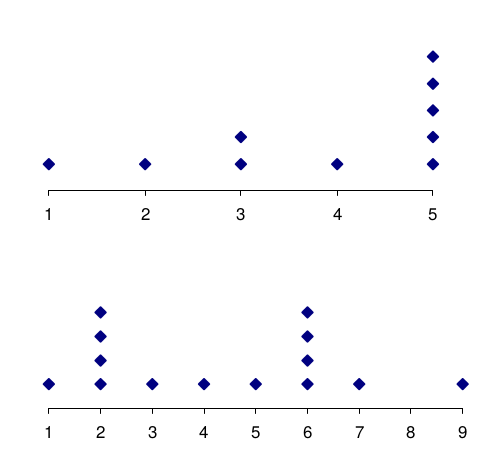
\includegraphics[height=0.7\textheight]{moda}
    \caption{Diagrama de pontos para dados (a) unimodal, (b) bimodal
      (Fonte: Reis, Reis, 2002)}
  \end{figure}
  % \begin{figure}
  %   \centering
  %   \pgfuseimage{moda2}
  % \end{figure}
\end{frame}

\subsection[Comparação]{Comparação entre as Medidas Centrais}

\begin{frame}{Comparação entre as Medidas Centrais}
  % \begin{figure}
  %   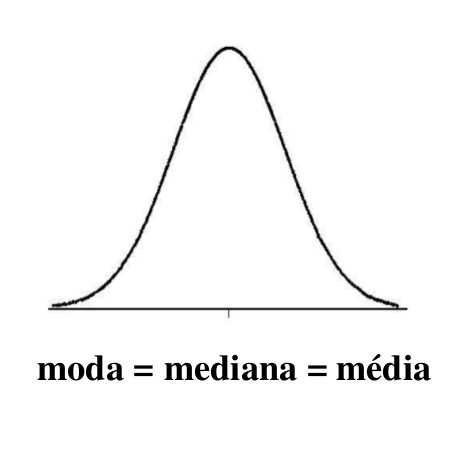
\includegraphics[height=0.3\textheight]{medidas1}
  %   \caption{Simétrica}
  % \end{figure}
  % \begin{figure}
  %   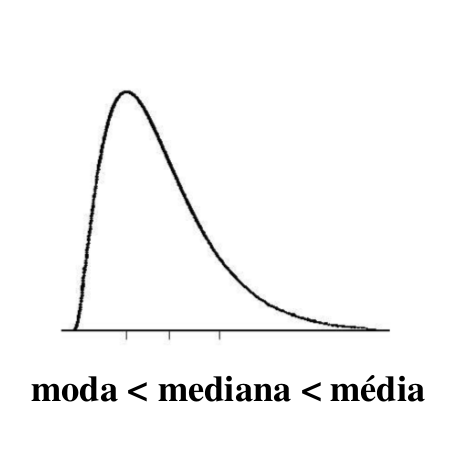
\includegraphics[height=0.3\textheight]{medidas2}
  %   \caption{Assimétrica à esquerda}
  % \end{figure}
  % \begin{figure}
  %   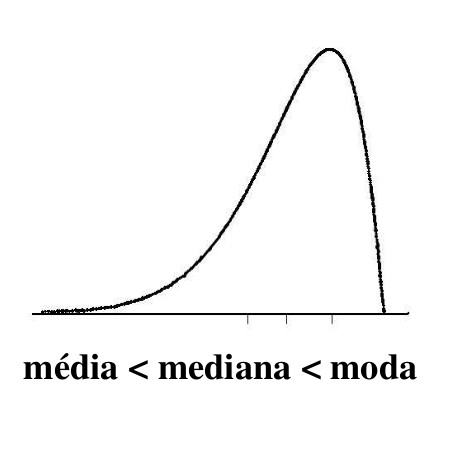
\includegraphics[height=0.3\textheight]{medidas3}
  %   \caption{Assimétrica à direita}
  % \end{figure}
    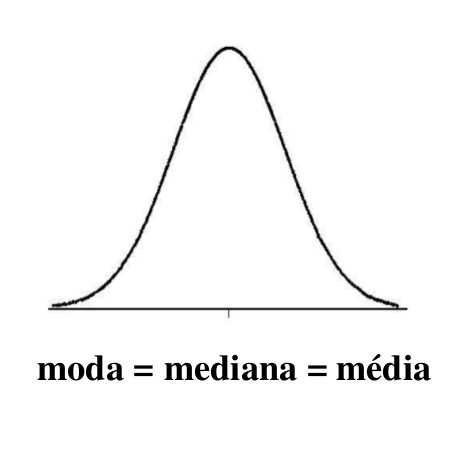
\includegraphics[height=0.4\textheight]{medidas1}
    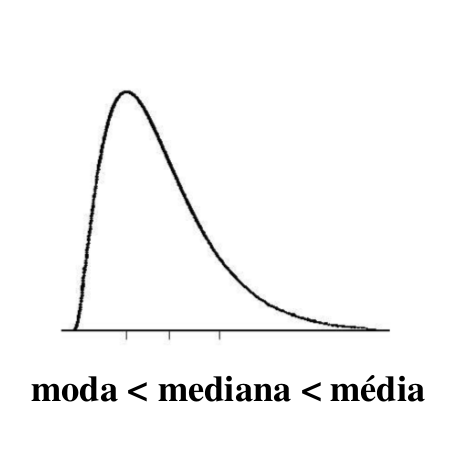
\includegraphics[height=0.4\textheight]{medidas2}
    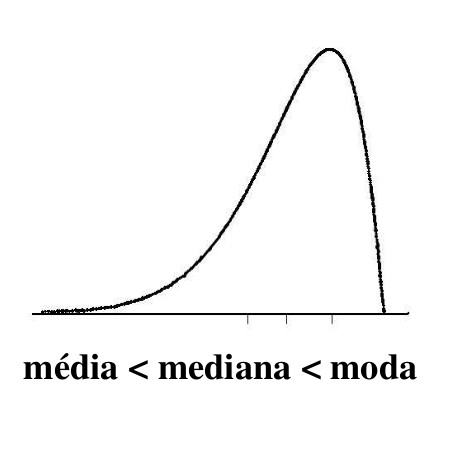
\includegraphics[height=0.4\textheight]{medidas3}
\begin{figure}
  \caption{(a) Simétrica, (b) Assimétrica à esquerda, (c) Assimétrica
    à direita (Fonte: Reis, Reis 2002)}
\end{figure}
\end{frame}

\begin{frame}{Robustez da Média}
  \begin{itemize}
  \item<1> A média é mais usada, mas não é \alert{robusta}.
  \item<1> É distorcida na presença de {\it outliers} (valores
    discrepantes, extremos)
%  \item<1> O que fazer nesta situação?
  \end{itemize}
  
\end{frame}
\begin{frame}{Comparação entre as Medidas Centrais}
  \begin{Example}Considere o seguinte dataset $$\{ 1,1,2,4,7\}$$
  \begin{itemize}
  \item $N=5$
  \item As medidas descritivas centrais para estes dados são:
  \item $\mu = \frac{1+1+2+4+7}{5} = \frac{15}{5}= 3$
  \item $M_d = 2$
  \item $M_o = 1$
  \end{itemize}
\end{Example}
\end{frame}

\begin{frame}{Comparação entre as Medidas Centrais}
  \begin{example}Considere agora este outro dataset $$\{
    1,1,2,4,32 \}$$
  \begin{itemize}
  \item $N=5$
  \item As medidas descritivas centrais para estes dados são:
  \item $\mu = \frac{1+1+2+4+32}{5} = \frac{40}{5}= 8$
  \item $M_d = 2$
  \item $M_o = 1$
  \end{itemize}
\end{example}
\end{frame}

%\subsection{Exercícios}
\begin{frame}{Exercícios}
  \begin{block}{Exercício}
    Um pesquisador observou as seguintes idades (anos) para uma amostra:
    35, 33, 37, 33, 34.
    
    Determine:
    \begin{enumerate}
    \item<1-> A média amostral ($\bar{x}$)
    \item<1-> A mediana ($M_d$)
    \item<1-> A moda ($M_o$)
    \end{enumerate}
  \end{block}
  
  \begin{block}{Solução}
    \begin{enumerate}
    \item $\bar{x} = \frac{35+33+37+33+34}{5} = 34.4$
    \item $M_d = 34$
    \item $M_o = 33$
    \end{enumerate}
  \end{block}
\end{frame}

\begin{frame}{Resumo}
  \begin{itemize}
  \item Média mais usual
  \item Mediana na presença de {\it outliers}
  \item Moda quando a distribuição das frequências for bimodal ou multimodal.
  \end{itemize}
  
\end{frame}

\section{Medidas de Dispersão}

\begin{frame}{Variabilidade em Medições}
  \begin{figure}
    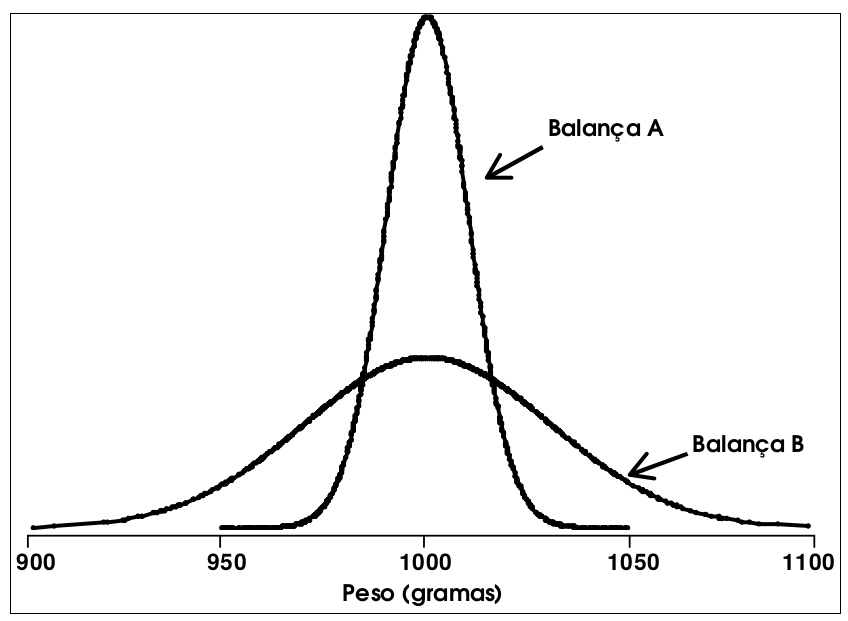
\includegraphics[height=0.7\textheight]{variancia}
    \caption{Variabilidade da medição de uma esfera metálica de
      1000g. Balança A, ``imprecisão'' de 50g, balança B,
      ``imprecisão'' de 100g (Fonte: Reis, Reis, 2002)}
  \end{figure}
\end{frame}

\subsection{Amplitude}
\begin{frame}{Amplitude}
  A amplitude dos dados identifica o intervalo de ocorrência de todos
  os dados observados
  \begin{itemize}
  \item $A = x_{max} - x_{min}$
  \end{itemize}
  \begin{example}
    Seja o dataset $$\{21, 12, 20, 4, 75, 40, 39, 63 \}$$

    Então, a amplitude é:
    % \begin{displaymath}
      $$A = 75 - 4 = 71$$
    % \end{displaymath}
  \end{example}
\end{frame}

\subsection{Desvios em relação à media}
\begin{frame}{Desvios em relação à média}
  \begin{itemize}
  \item Uma maneira de entender a variabilidade do dataset é analisar
    os desvios em relação à média.
  \item Cada desvio é a diferença entre o valor do dado e a média.
  % \item $D_j = x_j - \mu$ ou $D_i = x_i - \bar{x}$
  \end{itemize}
\end{frame}

\begin{frame}{Desvios em relação à média}
  Mas os desvios...
  \begin{enumerate}
  \item são tão numerosos quanto os dados
  \item têm sinal (direção do desvio)
  \item têm soma \alert{nula}
  \end{enumerate}
\end{frame}

\begin{frame}{Desvios em relação à média}
\begin{example}
  \begin{displaymath}
    \{1,2,3,4,5\}
  \end{displaymath}

  \begin{columns}
    \begin{column}{5cm}
  \begin{itemize}
  \item $N=5$
  \item $\bar{x} = 3$
  \end{itemize}
\end{column}
\begin{column}{5cm}
  \begin{enumerate}
  \item $D_1 = 1-3 = -2$
  \item $D_2 = 2-3 = -1$
  \item $D_3 = 3-3 = 0$
  \item $D_4 = 4-3 = 1$
  \item $D_5 = 5-3 = 2$
  \end{enumerate}
\end{column}
\end{columns}
\end{example}
\end{frame}

\begin{frame}{Soma dos desvios}
  \begin{example}
    Somando tudo:
    \begin{displaymath}
    D_1 + D_2 + D_3 + D_4 + D_5 =
  \end{displaymath}
  \begin{displaymath}
    (-2) + (-1) + 0 + 1 + 2 = 0
  \end{displaymath}
  \end{example}
\end{frame}

\begin{frame}{Como proceder?}
  \begin{itemize}
  \item Como extrair alguma informação útil (e sumária!) dos desvios?
  \item Problema: sinais
  \end{itemize}
  \begin{block}{Pergunta}
    Como tirar os sinais dos desvios?
  \end{block}
\end{frame}

\begin{frame}{Desvios absolutos}
  Tomando-se o módulo dos desvios temos:
  % \item Idéia matemática de ``tamanho''

  \begin{definition}
    Desvio médio absoluto (MAD) é a média dos desvios absolutos
  \end{definition}

  \begin{itemize}
  \item É uma medida de dispersão robusta (pouco influenciada por
    outliers)
  \item Módulo não tem boas propriedades matemáticas (analíticas e
    algébricas).
  \item Pouco usado para inferência (baixa eficiência)
  \end{itemize}
\end{frame}

\begin{frame}{Desvio médio absoluto (MAD)}
  \begin{example}
  \begin{displaymath}
    \{1,2,3,4,5\}, \bar{x} = 3
  \end{displaymath}
  \begin{columns}
    \begin{column}{5cm}<1->
      \begin{enumerate}
      \item $|D_1| = |1-3| = 2$
      \item $|D_2| = |2-3| = 1$
      \item $|D_3| = |3-3| = 0$
      \item $|D_4| = |4-3| = 1$
      \item $|D_5| = |5-3| = 2$
      \end{enumerate}
    \end{column}
    \begin{column}{5cm}
      \begin{displaymath}
        \mathrm{MAD } = \frac{\sum D_i}{5} = \frac{6}{5} = 1.2
      \end{displaymath}
    \end{column}
  \end{columns}
  \end{example}
\end{frame}

\begin{frame}{Uma proposta ``melhor''}
  \begin{itemize}
  \item Uma outra maneira de eliminar os sinais é elevar ao quadrado
    cada desvio.
  \item Preserva boas propriedades matemáticas
  \item Calculando a média dos quadrados dos desvios (desvios
    quadráticos) temos \ldots
  \end{itemize}
\end{frame}

\subsection{Variância}
\begin{frame}{Variância}
  \begin{definition}
    A variância é a média dos desvios quadráticos.
  \end{definition}
  \begin{itemize}
  \item Variância populacional
$$\sigma^2 = \frac{\sum (x_j - \mu)^2}{N}$$
\item Variância amostral
$$s^2 = \frac{\sum (x_i - \bar{x})^2}{n-1}$$
\item Conveniente do ponto de vista matemático (boas propriedades
  algébricas e analíticas).
\item Unidade quadrática, pouco intuitiva para interpretação de
  resultados.
  \end{itemize}
\end{frame}

\begin{frame}{Variância}
  \begin{example}
      \begin{displaymath}
    \{1,2,3,4,5\}, \bar{x} = 3
  \end{displaymath}
  \begin{columns}
    \begin{column}{6cm}<1->
      \begin{enumerate}
      \item $D_1^2 = (1-3)^2 = (-2)^2 = 4$
      \item $D_2^2 = (2-3)^2 = (-1)^2 = 1$
      \item $D_3^2 = (3-3)^2 = 0^2 =0$
      \item $D_4^2 = (4-3)^2 = 1^2 = 1$
      \item $D_5^2 = (5-3)^2 = 2^2 = 4 $
      \end{enumerate}
    \end{column}
    \begin{column}{4cm}
      \begin{displaymath}
        s^2 = \frac{\sum D_i^2}{4} = 2.5
      \end{displaymath}
    \end{column}
  \end{columns}
  \end{example}
\end{frame}

\subsection{Desvio Padrão}
\begin{frame}{Desvio Padrão}
  \begin{definition}
    O desvio padrão é a raiz quadrada da variância.
  \end{definition}
  \begin{itemize}
  \item Desvio padrão populacional
    $$ \sigma = \sqrt{ \sigma^2 } = \sqrt{ \frac{\sum (x_i - \mu)^2}{N} } $$
  \item Desvio padrão amostral
    $$ s = \sqrt{s^2 } = \sqrt{ \frac{\sum (x_i - \bar{x})^2}{n-1} } $$
  \end{itemize}
\end{frame}

\begin{frame}{Desvio Padrão}
  \begin{itemize}
  \item É a medida mais usada, por estar na mesma escala (unidade) dos
    dados.
  \item Boas propriedades matemáticas
  \item Boas propriedades como estimador (Inferência)
  \end{itemize}
\end{frame}

\begin{frame}{Desvio Padrão}
  \begin{example}
      \begin{displaymath}
    \{1,2,3,4,5\}, \bar{x} = 3
  \end{displaymath}
      \begin{displaymath}
        s^2 = 2.5
      \end{displaymath}
    \begin{displaymath}
        s = \sqrt{s^2} = \sqrt{2.5} = 1.58
    \end{displaymath}
  \end{example}
\end{frame}

\subsection{Exercícios}
\begin{frame}{Exercícios}
  \begin{block}{Exercício}
    Um pesquisador observou as seguintes idades (anos) para uma amostra:
    35, 33, 37, 33, 34.
    
    Determine:
    \begin{enumerate}
    \item<1-> A variância amostral ($s^2$)
    \item<1-> O desvio padrão amostral ($s$)
    \end{enumerate}
  \end{block}
  
  \begin{block}{Solução}
    Lembrando que $\bar{x} = 34.4$, temos:
    \begin{enumerate}
    \item $s^2 =
      % \frac{(35-34.4)^2+(33-34.4)^2+(37-34.4)^2+(33-34.4)^2+(34-34.4)^2}{5-1}
      \frac{(35-34.4)^2+(33-34.4)^2+\ldots}{5-1}$
      $=\frac{0.36+1.96+6.76+1.96+0.16}{4}=2.8$
    \item $s = \sqrt{2.8} = 1.67 $
    \end{enumerate}
  \end{block}
\end{frame}

\subsection{Coeficiente de Variação}
\begin{frame}{Coeficiente de Variação}
  \begin{definition}
    $$CV = \frac{\sigma}{\mu}$$
  \end{definition}
  \begin{itemize}
  \item Normaliza a variabilidade em relação à média
  \item Permite comparar a variabilidade de datasets não relacionados
    (mesmo que não usem a mesma unidade)
  \item Só deve ser usado para grandezas em escala (i.e. possui um
    ``zero'' não arbitrário, ou ``zero absoluto'')
  \end{itemize}
\end{frame}

\begin{frame}{Coeficiente de Variação}
  \begin{example}
    \begin{columns}<1->
      \begin{column}{5cm}<1->

        $x=$ Estatura e $y=$ Perímetro abdominal.

        \begin{tabular}{cc}
          $x=$ &$y=$\\
          \hline
          181.2 &76.3\\
          173.7&66.7\\
          169.0&73.3\\
          184.1&74.8\\
          174.4&82.7\\
          172.6&79.6\\
        \end{tabular}
      \end{column}
      \begin{column}{5cm}<1->

        Qual das duas amostras tem maior variabilidade?

        \begin{enumerate}
        \item Calcular a média $\bar{x}$
        \item Calcular a variância $s^2 = \frac{\sum (x_i - \bar{x})^2}{n-1}$
        \item Calcular o desvio padrão $s = \sqrt{s^2 }$
        \item $CV = \frac{s}{\bar{x}}$
        \end{enumerate}
      \end{column}
    \end{columns}
  \end{example}

\end{frame}

\begin{frame}{Coeficiente de Variação}
  \begin{example}
    \begin{columns}<1>
      \begin{column}{5cm}<1>

        $x=$ Estatura e $y=$ Perímetro abdominal.

        \begin{tabular}{cc}
          $x=$ &$y=$\\
          \hline
          181.2 &76.3\\
          173.7&66.7\\
          169.0&73.3\\
          184.1&74.8\\
          174.4&82.7\\
          172.6&79.6\\
        \end{tabular}
      \end{column}
      \begin{column}{5cm}<1>
        $\bar{x} = 175.8$
        $s_x = 5.7$

        $\bar{y} = 75.7$
        $s_y = 5.5$

        \alert{$CV_x = % \frac{5.7}{175.8} =
          3.24\%$}

        \alert{$CV_y = % \frac{5.5}{75.7} =
          7.27\%$}

        Resposta: O perímetro abdominal tem maior variabilidade que a
        altura.
      \end{column}
    \end{columns}
  \end{example}

\end{frame}

\section{Medidas de Posição}

\begin{frame}{Medidas de Posição}
  \begin{itemize}
  \item Permitem estabelecer informações quantitativas relativas à
    ordem dos dados
%  \item
  \end{itemize}
\end{frame}

\subsection{Quartis}
\begin{frame}{Quartis}
  \begin{definition}
    Dividem o dataset em quatro partes, cada uma com 25\% dos dados
  \end{definition}
  \begin{itemize}
  \item $Q_1$, primeiro quartil, representa os primeiros 25\% dos dados
  \item $Q_2$, segundo quartil, representa os primeiros 50\% dos dados
  \item $Q_3$, terceiro quartil, representa os primeiros 75\% dos dados
  \end{itemize}
  \begin{block}{Pergunta}
    O que podemos dizer sobre o segundo quartil ($Q_2$)?    
  \end{block}
\end{frame}

\begin{frame}{Quartis}
  \begin{example}
    Os pesos de $102$ bebês nascidos em uma certa maternidade ao longo
    de um ano foram anotados e ordenados. Um certo bebê ocupa o $Q_3$
    deste dataset.

    \begin{itemize}
    \item Isto significa que aproximadamente 75\% dos bebês nascidos nesta
    maternidade tem peso menor ou igual a ele (Mazel Tov!).
  \end{itemize}
\end{example}
\end{frame}

\subsection{Percentis e Decis}
\begin{frame}{Percentis e Decis}
  \begin{definition}
    O percentil de ordem $k$ (onde $k$ é qualquer valor entre 0 e
    100), denotado por $P_k$ , é o valor tal que $k\%$ dos valores do
    dataset são menores ou iguais a ele.
  \end{definition}

  \begin{itemize}
  \item Generalizam a idéia dos quartis
  \item Dividem o dataset em 100 partes
  \item Maior granularidade na ordem
  \item \alert{Decis}: dividem o dataset em 10 partes
  \end{itemize}
\end{frame}

% \subsection{Escore padrão}
% \begin{frame}{Escore padrão}
%   \begin{definition}
%   \end{definition}
%   \begin{itemize}
%   \item 
%   \end{itemize}
% \end{frame}

\section{Boxplot}
\begin{frame}{O Boxplot}
  \begin{itemize}
  \item Gráfico que ilustra a dispersão dos dados pelos quartis
  \item Retângulo que representa a Distância Interquartílica ($DQ =
    Q_3-Q_1$)
  \item Barra interna que representa a mediana ($Q_2$)
  \item Limite superior (barra vertical): $Q_3 + 1.5 \cdot DQ$
  \item Limite inferior (barra vertical): $Q_1 - 1.5\cdot DQ$
  \item Outliers como pontos, círculos ou estrelas
  \item Conveniente para comparar vários grupos ou amostras
  \end{itemize}
\end{frame}

\begin{frame}{O Boxplot}
  \begin{example}
    Dataset
    \begin{columns}
      \begin{column}{5cm}
        \begin{displaymath}
          \{1,2,3,4,5\}
        \end{displaymath}
        \begin{displaymath}
          \bar{x} = 3, M_d = 3
        \end{displaymath}
        \begin{displaymath}
          Q_1= 2, Q_3 = 4
        \end{displaymath}
      \end{column}
      \begin{column}{5cm}
        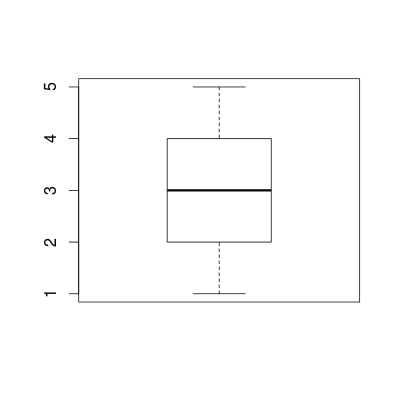
\includegraphics[height=0.6\textheight]{boxplot1}
      \end{column}
    \end{columns}
  \end{example}
\end{frame}

\begin{frame}{O Boxplot}
  \begin{example}
    \begin{columns}
      \begin{column}{5cm}
        Exemplo do colesterol
        \begin{tabular}{ccc}
          $x_1$ &=&142\\
          $x_2$ &=&144\\
          $x_3$ &=&176\\
          $x_4$ &=&203\\
          $x_5$ &=&134\\
          $x_6$ &=&191\\
        \end{tabular}
        $\bar{x}=165, M_d=160$
      \end{column}
      \begin{column}{5cm}
        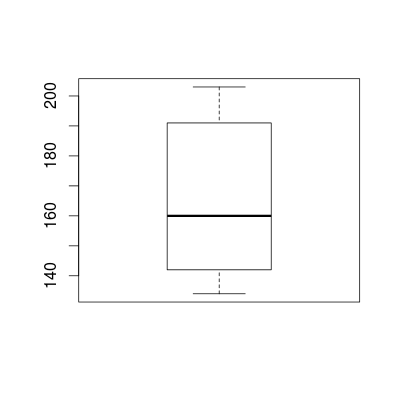
\includegraphics[height=0.6\textheight]{boxplot2}
      \end{column}
    \end{columns}
  \end{example}
\end{frame}

\begin{frame}{Boxplot: duas amostras}
  \begin{figure}
    \centering
    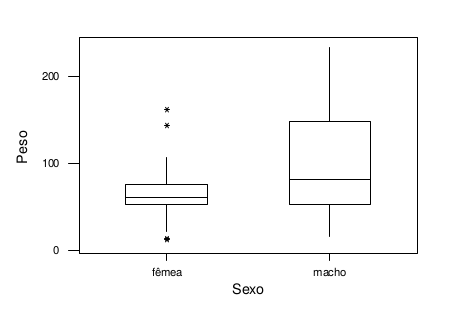
\includegraphics[height=0.7\textheight]{boxplot3}
    \caption{Boxplots para dois grupos de dados (Fonte: Reis, Reis,
      2002)}
  \end{figure}
\end{frame}

\section{Resumo}

\begin{frame}{Análise Exploratória de Dados (EDA)}
  Ao iniciar sua Análise Exploratória de Dados (EDA), você pode
  visualizar sua amostra com:
  \begin{enumerate}
  \item Resumo dos cinco números
    \begin{itemize}
    \item Valor mínimo
    \item Primeiro quartil $Q_1$
    \item Mediana (e/ou média)
    \item Terceiro quartil $Q_3$
    \item Valor máximo
    \end{itemize}
  \item Boxplot
  \end{enumerate}
  \begin{center}
  
\includegraphics[height=0.2\textheight]{protip}
  \end{center}
\end{frame}

\end{document}

